\documentclass[useAMS,usenatbib]{mn2e}

\usepackage{epsfig}
\usepackage{epstopdf}
\usepackage{lscape} % Allows landscape environment to be used
\usepackage{graphicx}
\usepackage{multirow}
\usepackage{hhline}
\usepackage{amsmath}
%\def\gtrsim{\mathrel{\hbox{\rlap{\hbox{\lower4pt\hbox{$\sim$}}}\hbox{$>$}}}}
%\renewcommand\floatpagefraction{.9}
%\renewcommand\dblfloatpagefraction{.9} % for two column documents
%\renewcommand\topfraction{.9}
%\renewcommand\dbltopfraction{.9} % for two column documents
%\renewcommand\bottomfraction{.9}
%\renewcommand\textfraction{.1}   
%\setcounter{totalnumber}{50}
%\setcounter{topnumber}{50}
%\setcounter{bottomnumber}{50}

\title[Lensing Distance]{
Precision Scintillation Distance Measurements
}
\author[Liu et al]{Siqi Liu$^{1,3}$\thanks{E-mail:\ sqliu@cita.utoronto.ca}, Ue-Li
  Pen$^{1,2}$\thanks{E-mail:\ pen@cita.utoronto.ca}, J-P Macquart$^{4}$\thanks{E-mail:J.Macquart@curtin.edu.au},
  Walter Brisken$^{5}$\thanks{Email:wbrisken@aoc.nrao.edu}, Adam Deller$^{6}$\thanks{E-mail:deller@astron.nl}\\
 $^1$ Canadian Institute for Theoretical Astrophysics, University of Toronto, M5S 3H8 Ontario, Canada \\
$^2$ Canadian Institute for Advanced Research, Program in Cosmology
and Gravitation\\
$^3$ Department of Astronomy and Astrophysics, University of Toronto, M5S 3H4, Ontario, Canada\\
$^4$ ICRAR-Curtin University of Technology, Department of Imaging and Applied Physics, GPO Box U1978, Perth, Western Australia 6102, USA \\
$^5$ National Radio Astronomy Observatory, P.O. Box O, Socorro, NM 87801, USA\\
$^6$ ASTRON, the Netherlands Institute for Radio Astronomy, Postbus 2, 7990 AA, Dwingeloo, The Netherlands\\
}
\begin{document}


\date{\today}

\pagerange{\pageref{firstpage}--\pageref{lastpage}} 
\pubyear{2015}

\maketitle
\label{firstpage}
\begin{abstract}
We show how interstellar scintillations, combined with VLBI
measurements, can be used to measure pulsar distances.  Two lensing
screens are needed.  We apply the technique to archival data on PSR
B0834+06.  Rough distance estimates, consistent with direct parallax
measurements, are obtained.  If observations over a six month period
had been made at that epoch, we anticipate a 1\% distance
determination.   

With longer ground-based baselines and wider frequency coverage, we
speculate that distance determination perhaps as accurate as 0.1\%
could be possible. This would enable coherent pulsar gravitational
wave timing and imaging.
\end{abstract}
\begin{keywords}
Pulsar
\end{keywords}

\newcommand{\be}{\begin{eqnarray}}
\newcommand{\ee}{\end{eqnarray}}
\newcommand{\beq}{\begin{equation}}
\newcommand{\eeq}{\end{equation}}

\section{Introduction}

Pulsars have long provided a rich source of astrophysical information
due to their compact emission and predictable timing.   One of the
weakest measurements for most pulsars is their direct geometric
distance.  For some pulsars, timing parallax or VLBI parallax has
resulted in direct distance determinations.  For most pulsars, the
distance is a major uncertainty for precision timing interpretations,
including mass, moment of inertia, and gravitational wave
direction\citep{boyle2012}.

Direct VLBI observation of PSR B0834+06 shows multiple images lensed
by the interstellar plasma.  Combining the angular positions and
scintillation delays, the authors published the derived effective
distance\citep{2010ApJ...708..232B} of approximately $1168\pm 23$ pc.
This represents a precise measurement compared to all other attempts
to derive distances to this pulsar.  This effective distance is a
combination of pulsar-screen and earth-screen distances, and does not
allow a separate determination of the individual distances.

A second lensing screen breaks the degeneracy.

\section{Lensing}
The previous result is that for $0.4$ms apexes data, the $D_{eff}=1168\pm 23$pc, and the $1$ms data , the $D_{eff}=1121\pm59$pc, which are degenerate.
To know the accurate position of the pulsar and the screen, we need to break this degeneracy.

This time, when we deal with the archival data. How distance is related to the time delay and how velocity is related to the differential frequency is defined by the following equations:

\begin{align*}
\tau &=\frac{D_{eff}{\theta}^2}{2c} \\
f_D  &=f*\frac{\delta\tau}{dt}
\end{align*} 

From $\tau$, RA and dec, we obtained the result that the positions of the pulsar: 
$0.4$ms ,$D_{eff}=1017\pm2.8$pc,
$1$ms, $D_{eff}=1121\pm64$pc
where the degeneracy is broken.Furthermore, if we know the distance of the pulsar is $640$pc by parallax,
the screen where $0.4$ms scintellation points are deflected, $D_s$ is equivalent to $392.82$pc. Then with the angle of the axis 25.2 degree west of north, we get the calculated RA and dec.

Similarly, for $1$ms pile, the $D_s$ is equivalent to $422.5$pc and calulated the RA and dec.
Then we fit a line to this five calculated points. Lying on the fitted line, point 5 is obtained with equal $\theta_{\parallel}$ as the farthest point in the 0.4ms pile. Knowing the fD of this point, we know the relative velocity of this point to the pulsar, which is called vA5. Similarly, we obtained the $v_{\parallel}$ from the 0.4ms data. Thus, the total velocity of the pulsar is determined.
Knowing tau, we can get the angle of the screen image away from the pulsar. Knowing the line and the differential frequency, we can get the ra and dec of the pulsar.

But accordign to Fermat's law, the distributions of the pile of 1ms points are not reasonable. If they are being reflected by one interstellar medium lens, they should be distributed along a line like the 0.4ms pile, just lie in the direction of the pulsar and point J in \ref{Doublelens}.

One alternative explanation of this is: the 1ms pile of points are the result of double lens. First deflected and then reflected. Solved positions are plotted in \ref{Doublelens}. By Fermat's law, the velocity parallel to the lens plane should be equal. 

We made a plot of the reflected velocity in the direction that is transverse to the first lens plane in \ref{vtrans}.


\section{B0834+06}


Our analysis is based on the reduced apex catalog from
\citet{2010ApJ...708..232B}. Each identified apex includes a delay,
delay rate, RA and Dec, one for each of 4 frequency bands.  We mapped
a total of 9 apexes from the 0.4ms cluster, and 5 from the 1ms
cluster, across the 4 frequency bands.  This results in an estimate
for the mean value, and standard deviation.  These are listed in Table
\ref{table:apex}. The time is calculated with $2{\tau}f/{f_{D}}$,
which is equivalent to pulsar moving at $640$pc plane from the
original position to the lensed image angle with the velocity
calculated. A least squares effective distance results in
$D_e^M=1017\pm 2.8$ for the main 0.4ms cluster and
$D_e^S = 1243 \pm 64.1$ for the secondary 1ms cluster.  This seems to
indicate that the secondary screen is closer to the pulsar.  The error
bars are large enough to allow them to be at the same distance, or
perhaps a reverse distance ordering.  In this paper, we present two
analyses for comparison: equidistant, and at the best fit distances.
In the first case, no direct distance measurement is possible, but it
nevertheless illustrates a robust interpretation of the data.

%table one for 1ms positions

\begin{table*}
\centering
%\label{apex1ms}
%\resizebox{!}{1cm}{
\begin{tabular}{|c|c|c|c|c|c|c|c|c|}
\hline
$f_D$(mHz) & $\sigma_{f_D}$(mHz) & $\tau$(ms) & $\sigma_{\tau}$(ms) & RA(mas) & $\sigma_{RA}$(mas) & dec(mas) & $\sigma_{dec}$(mas) & time(day)\\
\hline
-12.94                            & 0.19      & 0.0845  & 0.0005          & 2.87    & 0.11                                     & -8.2     & 0.09      & 49.9                                \\

-16.8                             & 0.28      & 0.14125 & 0.00085         & 3.86    & 0.07                                     & -10.6    & 0.05      &64.5                                \\

-18.92                            & 0.23      & 0.188   & 0.002           & 5.06    & 0.2                                      & -10.6    & 0.13      &74.4                        \\

-20.4                             & 0.49      & 0.222   & 0.003           & 5.55    & 0.3                                      & -11.7    & 0.21      &80.8                                \\

-21.17                            & 0.61      & 0.236   & 0.002           & 5.12    & 0.43                                     & -12.6    & 0.31      &83.4                                \\

-22.32                            & 0.47      & 0.2633  & 0.0003          & 6.16    & 0.14                                     & -14.2    & 0.1       &88.0                                \\

-24.63                            & 0.4       & 0.3265  & 0.0025          & 6.49    & 0.29                                     & -14.1    & 0.2       &98.0                                \\

-24.94                            & 0.44      & 0.33775 & 0.00025         & 8.29    & 0.42                                     & -14.4    & 0.32      &99.7                                \\

-26.09                            & 0.36      & 0.37425 & 0.00063         & 8.53    & 0.52                                     & -15.7    & 0.42      &105                               
\\ \hline 
-35.06                           & 0.52                               & 0.95               & 0.002                              & -15.23  & 0.69                                     & -21.06   & 0.7   &202                                   \\

-38.31                           & 0.64                               & 0.976              & 0.0009                             & -15.02  & 0.485                                    & -20.74   & 0.38  &190                                    \\

-40.17                           & 0.55                               & 1.005              & 0.0079                             & -14.14  & 0.662                                    & -22.27   & 0.62  &187                                   \\

-41.27                           & 0.54                               & 1.037              & 0.003                              & -11.28  & 0.93                                     & -19.18   & 1.1   &188                                   \\

-43.08                           & 0.44                               & 1.066              & 0.005                              & -8.41   & 1.7                                      & -24.14   & 1.4   &185   
                                  
\end{tabular}
\label{table:apex}
\caption{0.4ms and 1ms observation positions.}
\end{table*}



%\begin{figure*}
%\centering
%\epsscale{1.0}
%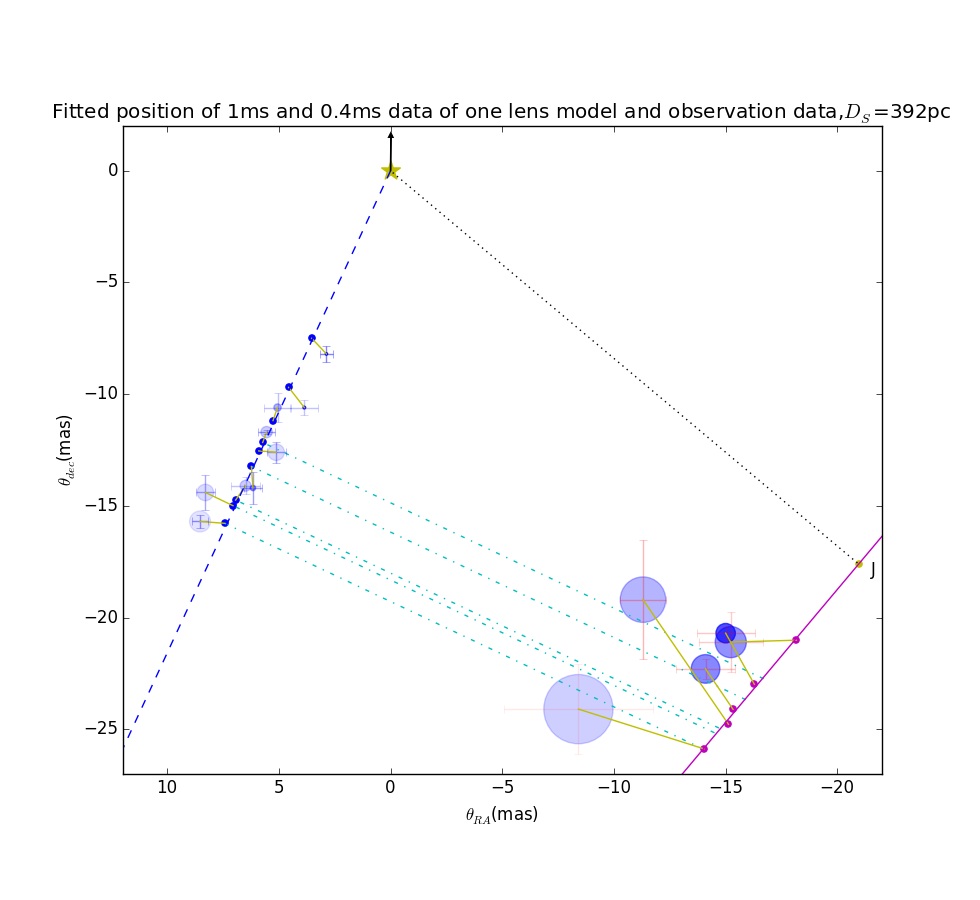
\includegraphics[width=0.8\textwidth, angle=0]{One_lens_640_392_392.png}
%\includegraphics{zN.eps}
%\caption{Fitted position of $1$ms and $0.4$ms data of one lens model and observation data. In both apexes regions, the position of the screen locate at $392.82$pc. Blue points on the left side are the points that fitted from the $f_D$ and $\tau$ of from the $0.4$ms observation. Blue line is the fitted line of $0.4$ms apex positions, with a $25.2$ degree west of the north. The points lie on the left side with errorbars, are the observation points together with their sample errors; while the transparent circles are plotted with population errors, where smaller transparent data are darker. Short solid lines between them are the matched positions of the apexes in $1ms$ region and $0.4ms$ region, which share the same $\theta_{\parallel}$. The points on the right side are the points that fitted from the $f_D$ and $\tau$ of the $1$ms observation with an avearage of four bandwidths. Solid line is the fitted line of these positions. Those points with errorbars nearby are the observation points together with their sample errors, while the transparent circles are plotted with population errors. The dotted line on the top right side is vertical to the solid line. Short solid lines connect the observation points and the fitted positions. Middle lines connect the $0.4$ms and $1$ms fitted positions with the same $\theta_{\parallel}$. The velocity of the pulsar is $199981$m/s, with a degree $0.0007$ radian east of north, which is marked out at the top of the figure.  }
%\label{Onelens_392}
%\end{figure*}

%\begin{figure*}
%\centering
%\epsscale{1.0}
%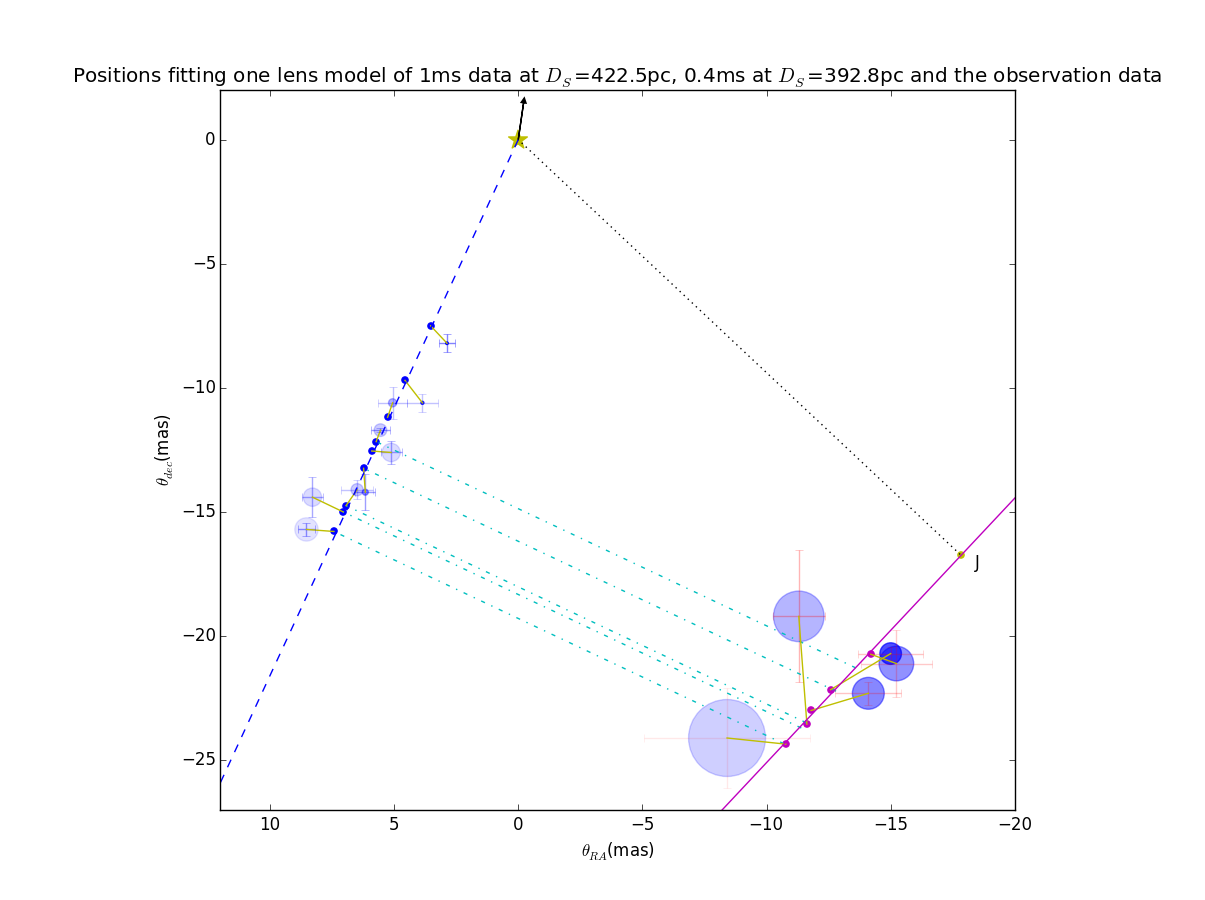
\includegraphics[width=0.8\textwidth, angle=0]{One_lens_640_392_422.png}
%\includegraphics{zN.eps}
%\caption{Same Observation data with the previous plot, this time we put the points with time delay lie in the range $1$ms at the screen that is $422.5$ pc away from us, which fitts better with the observation data. Velocity in this situation is $188499$m/s, with an angle $0.144147$ radian west of north. }
%\label{Onelens_392_422}
%\end{figure*}

\begin{figure*}
\centering
%\epsscale{1.0}
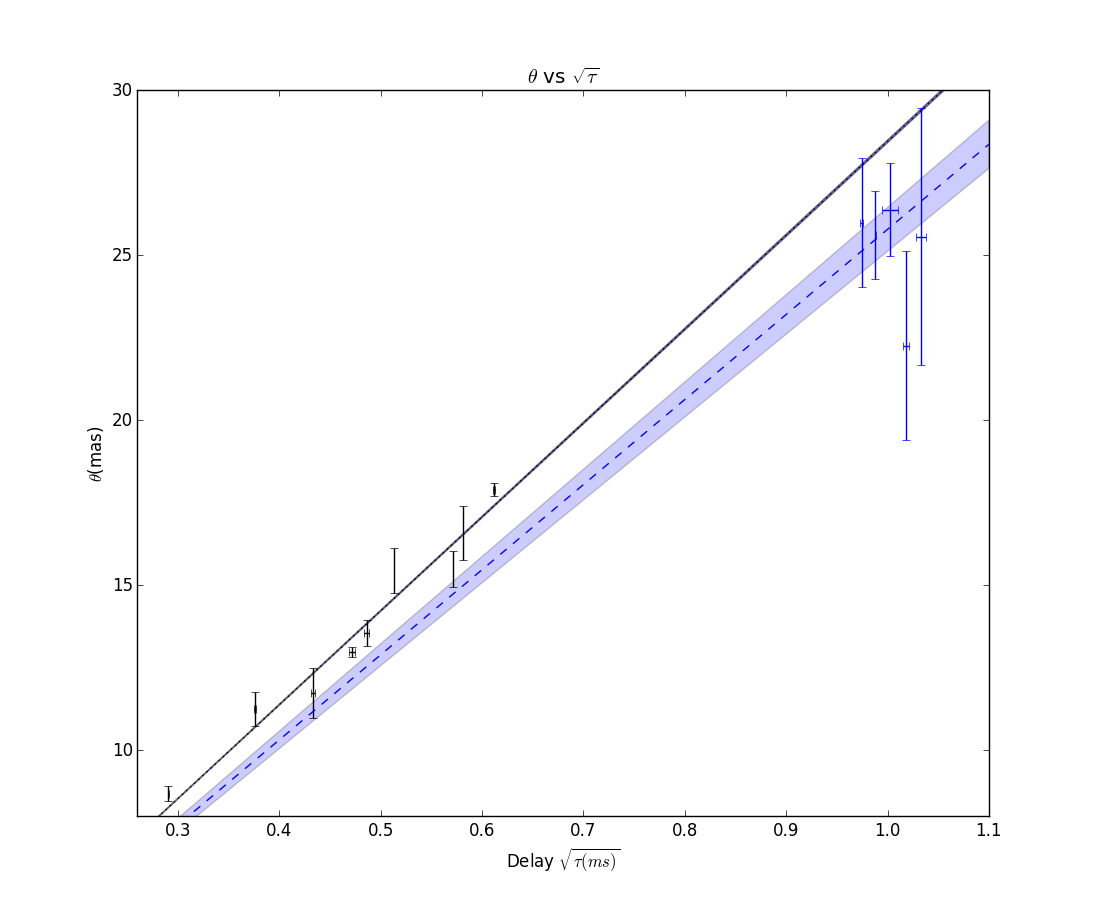
\includegraphics[width=1.0\textwidth, angle=0]{Theta_tau.png}
\caption{${\theta}$ vs ${\sqrt{\tau}}$. The black line is the fitted line of the 0.4ms positions, where $k=28.51$. The blue lines are the fitted lines of the 1ms position, where $k=25.784$ with an error region of $\sigma_k=0.66$.
}
\end{figure*}





\section{Lens Solution}

In order to interpret the data, we adopt the lensing model of
\citet{2014MNRAS.442.3338P}.  In the absence of a lens model, the
fringe rate, delay and angular position cannot be uniquely related. In
this model, the lensing is due to projected fold caustics of a thin
sheet closely aligned to the line of sight.


\begin{figure*}
\centering
%\epsscale{1.0}
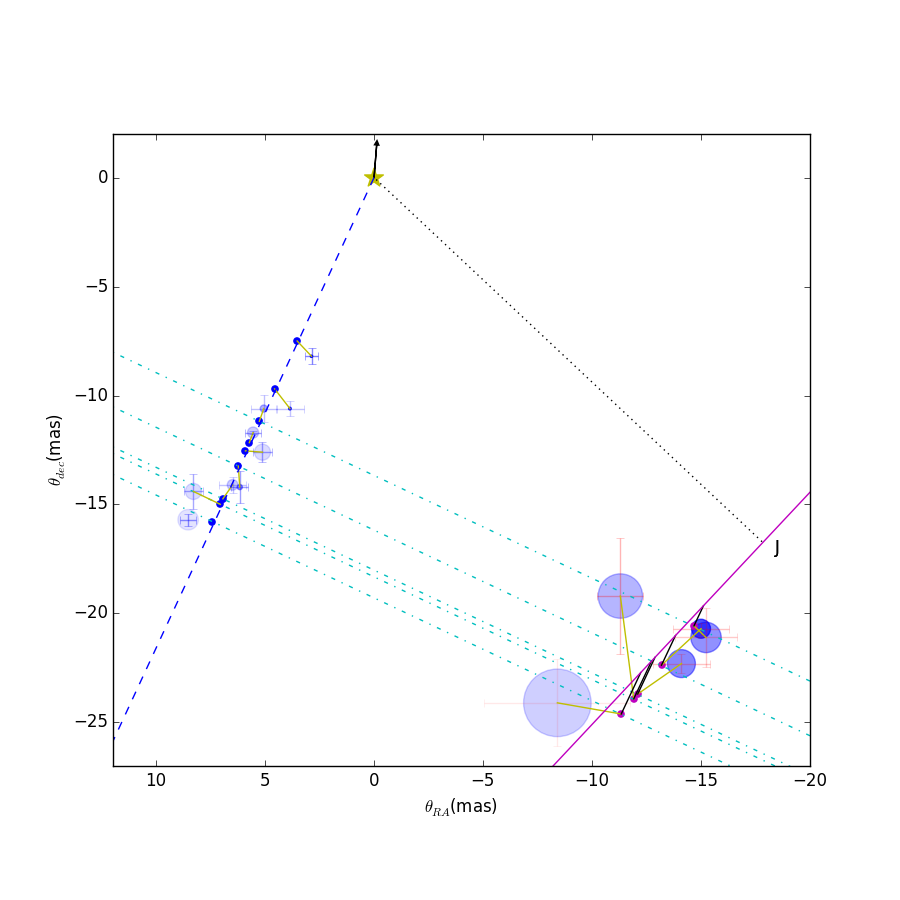
\includegraphics[width=1.0\textwidth, angle=0]{Double_lens_640_425_392.png}
\caption{Fitted position of $1$ms and $0.4$ms data of double lens model and observation data.In both apexes regions, the position of the screen locate at $392.82$pc and $425$pc. Blue points on the left side are the points that fitted from the $f_D$ and $\tau$ of from the $0.4$ms observation. Blue line is the fitted line of $0.4$ms apex positions, with a $25.2$ degree west of the north. The points lie on the left side with errorbars, are the observation points together with their sample errors; while the transparent circles are plotted with population errors, where smaller transparent data are darker. Short solid lines between them are the matched positions of the apexes in $1ms$ region and $0.4ms$ region, which share the same $\theta_{\parallel}$. The points on the right side are the points that fitted from the $f_D$ and $\tau$ of the $1$ms observation with an avearage of four bandwidths. Solid line is the fitted line of these positions. Those points with errorbars nearby are the observation points together with their sample errors, while the transparent circles are plotted with population errors. The dotted line on the top right side is vertical to the solid line. Short solid lines connect the observation points and the fitted positions. Middle lines connect the $0.4$ms and $1$ms fitted positions with the same $\theta_{\parallel}$. The velocity of the pulsar is $191.4$km/s, with a degree $5.56$ degree west of north, is also marked out at the top of the figure.  }
\label{Doublelens}
\end{figure*}



\begin{figure*}
\centering
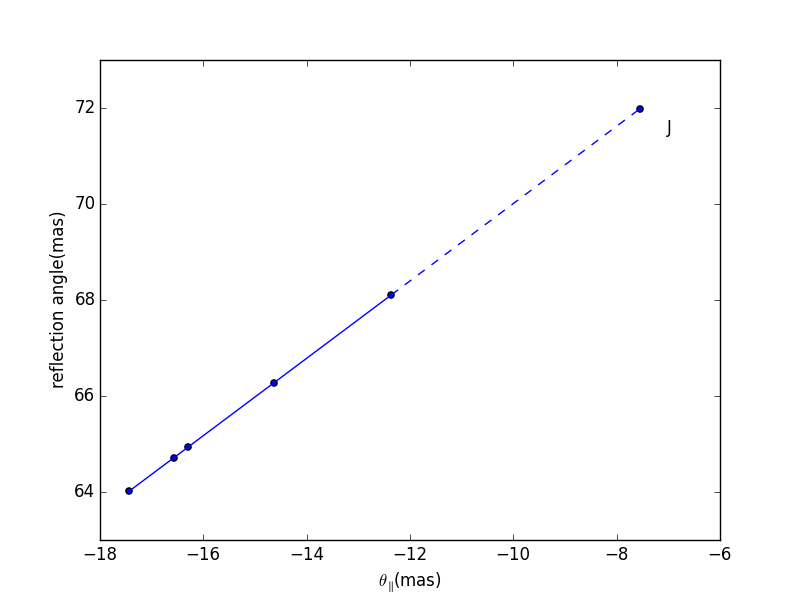
\includegraphics[width=1.0\textwidth,angle=0]{Reflection_angle.png}
\caption{Injection velocity minus reflected velocity over the speed of light. J specifically marked in the paper.}
\label{vtrans}
\end{figure*}

\section{Discussion}

The lens solution appears consistent with the premise of the inclined
sheet lensing model\citep{2014MNRAS.442.3338P}.  The secondary lens
only images a subset of the primary lens images.  This could happen if
the secondary lens screen is just under the critical inclination
angle, such that only $3-\sigma$ waves lead to a fold caustic.  If the
primary lens were at a critical angle, the chance of encountering a
somewhat less inclined system is of order unity.

More surprising is the absence of a single deflection image of the
pulsar, which is expected at position J.  This could happen if the
maximum deflection angle is just below critical, such that only rays
on the appropriately aligned double deflection can form images.  This
scenario predicts that at frequencies just below 300 MHz, or a few
weeks earlier in time, the pulsar should be seen at position J.

\section{Possible Improvements}

We discuss several strategies which can improve on the solution
accuracy.  The single biggest improvement would be to monitor over a
week, when the pulsar crosses each individual lens, including both
lensing systems.

Angular resolution can be improved using longer baselines, for example
adding a GMRT-GBT baseline doubles the resolution.  Observing at
multiple frequencies over a longer period allows for a more precise
measurement: when the pulsar is between two lenses, the deflection
angle is small, and one expects to see the lensing at higher
frequency, where the resolution is higher, and distances between
lenses positions can be measured to much higher accuracy.

Holographic techniques\citep{2008MNRAS.388.1214W,2014MNRAS.440L..36P}
may be able to measure delays, fringe rates, and VLBI positions
sbstantially more accurately.  Combining these techniques, the
interstellar lensing could conceivably achieve distance measurements
an order of magnitude better than the current published effective
distance errors.  This could bring most pulsar timing array targets
into the coherent timing regime, enabling arc minute localization of
gravitational wave sources, lifting any potential source confusion.

Ultimately, the precision of the lensing results would be limited by
the fidelity of the lensing model.  In the inclined sheet model, the
images move along fold caustics.  The straightness of these caustics
depends on the inclination angle, which in turn depends on the
amplitude of the surface waves.

\section{Conclusions}

We have presented a new technique of two plane interstellar plasma
lensing to determine distances to pulsars.  We have tested this
approach on archival data, showing that in principle solutions can be
obtained.  We conclude that multi-epoch observations over weeks, at a
range of frequencies, might result in much more accurate distance
determinations.


\section{Acknowledgements}

We thank NSERC for support.


\newcommand{\araa}{ARA\&A}   % Annual Review of Astronomy and Astrophys.
\newcommand{\afz}{Afz}       % Astrofizica
\newcommand{\aj}{AJ}         % Astronomical Journal
\newcommand{\azh}{AZh}       % Astronomicekij Zhurnal
\newcommand{\aaa}{A\&A}      % Astronomy and Astrophysics
\newcommand{\aas}{A\&AS}     % Astronomy and Astrophys. Supplement Series
\newcommand{\aar}{A\&AR}     % Astronomy and Astrophysics Review
\newcommand{\apj}{ApJ}       % Astrophysical Journal
\newcommand{\apjs}{ApJS}     % Astrophysical Journal Supplement Series
\newcommand{\apjl}{ApJ}      % Astrophysical Journal Letters
\newcommand{\apss}{Ap\&SS}   % Astrophysics and Space Science
\newcommand{\baas}{BAAS}     % Bulletin of the American Astron. Society
\newcommand{\jaa}{JA\&A}     % Journal of Astronomy and Astrophysics
\newcommand{\mnras}{MNRAS}   % Monthly Notices of the Roy. Astron. Society
\newcommand{\nat}{Nat}       % Nature
\newcommand{\pasj}{PASJ}     % Publ. of the Astron. Society of Japan
\newcommand{\pasp}{PASP}     % Publ. of the Astron. Society of the Pacific
\newcommand{\paspc}{PASPC}   % Publ. Astron. Soc. Pacific Conf. Proc.
\newcommand{\qjras}{QJRAS}   % Quart. Journal of the Royal Astron. Society
\newcommand{\sci}{Sci}       % Science
\newcommand{\solphys}{Solar Physics}       % 
\newcommand{\sova}{SvA}      % Soviet Astronomy
\newcommand{\aap}{A\&A}
\newcommand\jcap{{J. Cosmology Astropart. Phys.}}%
\newcommand{\prd}{Phys. Rev. D}


\bibliography{distance}
\bibliographystyle{mn2e}


\label{lastpage}

\end{document}
